%----------------------------------------------------------------------------------------
%	PACKAGES AND OTHER DOCUMENT CONFIGURATIONS
%----------------------------------------------------------------------------------------

\documentclass[18pt]{extarticle}

%%%%%%%%%%%%%%%%%%%%%%%%%%%%%%%%%%%%%%%%%
% Lachaise Assignment
% Structure Specification File
% Version 1.0 (26/6/2018)
%
% This template originates from:
% http://www.LaTeXTemplates.com
%
% Authors:
% Marion Lachaise & François Févotte
% Vel (vel@LaTeXTemplates.com)
%
% License:
% CC BY-NC-SA 3.0 (http://creativecommons.org/licenses/by-nc-sa/3.0/)
% 
%%%%%%%%%%%%%%%%%%%%%%%%%%%%%%%%%%%%%%%%%

%----------------------------------------------------------------------------------------
%	PACKAGES AND OTHER DOCUMENT CONFIGURATIONS
%----------------------------------------------------------------------------------------

\setlength{\parindent}{0em}
\setlength{\parskip}{.5em}

\usepackage{amsmath,amsfonts,stmaryrd,amssymb} % Math packages

\usepackage{enumerate} % Custom item numbers for enumerations

\usepackage[ruled]{algorithm2e} % Algorithms

\usepackage[framemethod=tikz]{mdframed} % Allows defining custom boxed/framed environments

\usepackage{dirtytalk}

\usepackage{listings} % File listings, with syntax highlighting
\lstset{
	basicstyle=\ttfamily, % Typeset listings in monospace font
}

\usepackage{hyperref}
\hypersetup{
    colorlinks=true,
    linkcolor=blue,
    filecolor=magenta,      
    urlcolor=cyan,
}


%----------------------------------------------------------------------------------------
%	DOCUMENT MARGINS
%----------------------------------------------------------------------------------------

\usepackage{geometry} % Required for adjusting page dimensions and margins

\geometry{
	paper=a4paper, % Paper size, change to letterpaper for US letter size
	top=2.5cm, % Top margin
	bottom=3cm, % Bottom margin
	left=2.5cm, % Left margin
	right=2.5cm, % Right margin
	headheight=14pt, % Header height
	footskip=1.5cm, % Space from the bottom margin to the baseline of the footer
	headsep=1.2cm, % Space from the top margin to the baseline of the header
	%showframe, % Uncomment to show how the type block is set on the page
}

%----------------------------------------------------------------------------------------
%	FONTS
%----------------------------------------------------------------------------------------

\usepackage[utf8]{inputenc} % Required for inputting international characters
\usepackage[T1]{fontenc} % Output font encoding for international characters

\usepackage{XCharter} % Use the XCharter fonts

%----------------------------------------------------------------------------------------
%	COMMAND LINE ENVIRONMENT
%----------------------------------------------------------------------------------------

% Usage:
% \begin{commandline}
%	\begin{verbatim}
%		$ ls
%		
%		Applications	Desktop	...
%	\end{verbatim}
% \end{commandline}

\mdfdefinestyle{commandline}{
	leftmargin=10pt,
	rightmargin=10pt,
	innerleftmargin=15pt,
	middlelinecolor=black!50!white,
	middlelinewidth=2pt,
	frametitlerule=false,
	backgroundcolor=black!5!white,
	frametitle={Command Line},
	frametitlefont={\normalfont\sffamily\color{white}\hspace{-1em}},
	frametitlebackgroundcolor=black!50!white,
	nobreak,
	singleextra={%
    }
}

% Define a custom environment for command-line snapshots
\newenvironment{commandline}{
	\medskip
	\begin{mdframed}[style=commandline]
}{
	\end{mdframed}
	\medskip
}

%----------------------------------------------------------------------------------------
%	FILE CONTENTS ENVIRONMENT
%----------------------------------------------------------------------------------------

% Usage:
% \begin{file}[optional filename, defaults to "File"]
%	File contents, for example, with a listings environment
% \end{file}

\mdfdefinestyle{file}{
	innertopmargin=1.6\baselineskip,
	innerbottommargin=0.8\baselineskip,
	topline=false, bottomline=false,
	leftline=false, rightline=false,
    leftmargin=0cm,rightmargin=0cm,
	singleextra={%
		\draw[fill=black!10!white](P)++(0,-1.2em)rectangle(P-|O);
		\node[anchor=north west]
		at(P-|O){\ttfamily\mdfilename};
		%
		\def\l{3em}
		\draw(O-|P)++(-\l,0)--++(\l,\l)--(P)--(P-|O)--(O)--cycle;
		\draw(O-|P)++(-\l,0)--++(0,\l)--++(\l,0);
	},
	firstextra={%
		\draw[fill=black!10!white](P)++(0,-1.2em)rectangle(P-|O);
		\node[anchor=north west]
		at(P-|O){\ttfamily\mdfilename};
		%
	},
    middleextra={%
    },
    secondextra={%
		\def\l{3em}
		\draw(O-|P)++(-\l,0)--++(\l,\l)--(P)--(P-|O)--(O)--cycle;
		\draw(O-|P)++(-\l,0)--++(0,\l)--++(\l,0);
    },
    nobreak,
}

% Define a custom environment for file contents
\newenvironment{file}[1][File]{ % Set the default filename to "File"
	\medskip
	\newcommand{\mdfilename}{#1}
	\begin{mdframed}[style=file]
}{
	\end{mdframed}
	\medskip
}

%----------------------------------------------------------------------------------------
%	NUMBERED QUESTIONS ENVIRONMENT
%----------------------------------------------------------------------------------------

% Usage:
% \begin{question}[optional title]
%	Question contents
% \end{question}

\mdfdefinestyle{question}{
	innertopmargin=1.2\baselineskip,
	innerbottommargin=0.8\baselineskip,
	roundcorner=5pt,
	singleextra={%
		\draw(P-|O)node[xshift=1em,anchor=west,fill=white,draw,rounded corners=5pt]{%
		Άσκηση \theQuestion\questionTitle};
	},
	firstextra={%
		\draw(P-|O)node[xshift=1em,anchor=west,fill=white,draw,rounded corners=5pt]{%
		Άσκηση \theQuestion\questionTitle};
	},
}

\newcounter{Question} % Stores the current question number that gets iterated with each new question

% Define a custom environment for numbered questions
\newenvironment{question}[1][\unskip]{
	\bigskip
	\stepcounter{Question}
	\newcommand{\questionTitle}{~#1}
	\begin{mdframed}[style=question]
}{
	\end{mdframed}
	\medskip
}

%----------------------------------------------------------------------------------------
%	WARNING TEXT ENVIRONMENT
%----------------------------------------------------------------------------------------

% Usage:
% \begin{warn}[optional title, defaults to "Warning:"]
%	Contents
% \end{warn}

\mdfdefinestyle{warning}{
	topline=false, bottomline=false,
	leftline=false, rightline=false,
	nobreak,
	singleextra={%
		\draw(P-|O)++(-0.5em,0)node(tmp1){};
		\draw(P-|O)++(0.5em,0)node(tmp2){};
		\fill[black,rotate around={45:(P-|O)}](tmp1)rectangle(tmp2);
		\node at(P-|O){\color{white}\scriptsize\bf !};
		\draw[very thick](P-|O)++(0,-1em)--(O);%--(O-|P);
	}
}

% Define a custom environment for warning text
\newenvironment{warn}[1][Warning:]{ % Set the default warning to "Warning:"
	\medskip
	\begin{mdframed}[style=warning]
		\noindent{\textbf{#1}}
}{
	\end{mdframed}
}

%----------------------------------------------------------------------------------------
%	INFORMATION ENVIRONMENT
%----------------------------------------------------------------------------------------

% Usage:
% \begin{info}[optional title, defaults to "Info:"]
% 	contents
% 	\end{info}

\mdfdefinestyle{info}{%
	topline=false, bottomline=false,
	leftline=false, rightline=false,
	nobreak,
	singleextra={%
		\fill[black](P-|O)circle[radius=0.4em];
		\node at(P-|O){\color{white}\scriptsize\bf i};
		\draw[very thick](P-|O)++(0,-0.8em)--(O);%--(O-|P);
	}
}

% Define a custom environment for information
\newenvironment{info}[1][Info:]{ % Set the default title to "Info:"
	\medskip
	\begin{mdframed}[style=info]
		\noindent{\textbf{#1}}
}{
	\end{mdframed}
}

\newcommand{\src}[1]{{\texttt{#1}}}

 % Include the file specifying the document structure and custom commands

%----------------------------------------------------------------------------------------
%	ASSIGNMENT INFORMATION
%----------------------------------------------------------------------------------------

\title{Εργασία Δημιουργίας Character Device Driver στο Linux Kernel \\Λειτουργικά Συστήματα (ECE ΓΚ702)} % Title of the assignment

% \author{\footnotesize Χρήστος Φείδας\\ \footnotesize \src{fidas@upatras.gr} \and \footnotesize Ευάγγελος Λάμπρου\\ \footnotesize \src{e.lamprou@upnet.gr}} % Author name and email address

\date{University of Patras, Department of Electrical and Computer Engineering} % University, school and/or department name(s) and a date

\usepackage{fancyhdr}
\usepackage{float}
\usepackage[main=greek, english]{babel}

%----------------------------------------------------------------------------------------

\begin{document}

\pagestyle{fancy}
%... then configure it.
\fancyhf{} % sets both header and footer to nothing
\renewcommand{\headrulewidth}{0pt}
\fancyhead{} % clear all header fields
\fancyfoot{} % clear all footer fields
\fancyfoot[L]{\footnotesize Χρήστος Φείδας, \footnotesize Ευάγγελος Λάμπρου}
\fancyfoot[R]{\thepage}

\maketitle

\tableofcontents

%----------------------------------------------------------------------------------------
%	INTRODUCTION
%----------------------------------------------------------------------------------------

\section{Εισαγωγή}

Στην εργασία αυτή θα γίνει μία παρουσίαση της διεπαφής με την οποία μία συσκευή επικοινωνεί με το λειτουργικό σύστημα. 
Θα εστιάσουμε στον τρόπο όπου ένας οδηγητής συσκευής (device driver) επικοινωνεί με το υπόλοιπο σύστημα σε περιβάλλον Linux.
Τέλος, θα δημιουργήσουμε στο σύστημά μας μια εικονική συσκευή για την οποία θα φτιάξουμε έναν απλό driver μέσω του οποίου θα μπορεί ένας χρήστης να αλληλεπιδράσει με αυτή.

Στο λειτουργικό σύστημα UNIX, πάνω στο οποίο είναι βασισμένο το Linux υπάρχει η ιδέα του \href{https://en.wikipedia.org/wiki/Everything_is_a_file}{"όλα είναι ένα αρχείο".}
Αυτό σημαίνει πως η επικοινωνία με περιφερειακές συσκευές όπως ένα πληκτρολόγιο μπορούμε να τις μοντελοποιήσουμε στο σύστημά μας σαν ροές από bytes.
Με άλλα λόγια, μπορούμε να φανταστούμε τις συσκευές σαν απλά αρχεία κειμένου, όπου το \say{κείμενο} σε αυτή την περίπτωση είναι τα δεδομένα της συσκευής.
Προγράμματα χρήστη στη συνέχεια μπορούν να επικοινωνήσουν με τη κάθε συσκευή διαβάζοντας ή γράφοντας στο αρχείο συσκευής (device file) που της αντιστοιχεί.
Η διεπαφή γίνεται μέσω κλήσεων συστήματος (system calls) όπως \src{open}, \src{read}, \src{write}, \src{close}, \src{lseek} κλπ.
Το λειτουργικό σύστημα μεσολαβεί αυτής της επικοινωνίας εκτελώντας τις ρουτίνες που προσφέρονται από τον driver της εκάστοτε συσκευής.
Ο κάθε driver είναι μέρος του kernel και μπορεί είτε να είναι ενσωματωμένος στον κώδικα του kernel είτε να φορτώνεται δυναμικά ως kernel module.

\begin{info}[Σημείωση]
    Μπορείτε να βρείτε περισσότερες πληροφορίες για τα system calls που είναι διαθέσιμα στο σύστημά σας διαβάζοντας τα αντίστοιχα \href{https://man7.org/linux/man-pages/dir_section_2.html}{manual pages}.
    Χρησιμοποιήστε και την εντολή \src{man} (πχ \src{man 2 open}).
\end{info}

\begin{figure}[htpb]
    \centering
    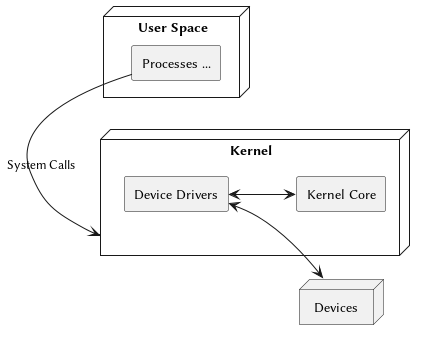
\includegraphics[width=.7\textwidth]{assets/drivers.png}
    \caption{Η επικοινωνία εφαρμογών χρήστη με συσκευές μέσω λειτουργικού συστήματος και των drivers.}
    \label{fig:drivers}
\end{figure}



% \section{Character/Block Devices}
% character/block devices


\section{Αρχεία Συσκευών (Device Files)}

Όπως είπαμε, κάθε φυσική συσκευή που υπάρχει στο σύστημά σας έχει ένα (ή περισσότερα) αρχείο συσκευής που της αντιστοιχεί. 
Μέσω αυτού μπορούν διεργασίες στο σύστημα να αλληλεπιδράσουμε με τη συσκευή.
Σε UNIX-like συστήματα, οι συσκευές βρίσκονται συνήθως στον φάκελο \src{/dev}.
Αυτό είναι μια αυθαίρετη επιλογή και υπάρχει για λόγους οργάνωσης.

Επισκεφθείτε τον φάκελο \src{/dev} και δείτε τα αρχεία συσκευών που υπάρχουν εκεί. 
Μπορείτε να τα δείτε χρησιμοποιώντας και την παρακάτω εντολή.

\begin{commandline}
\begin{verbatim}
$ ls -la /dev/sd? /dev/random
crw-rw-rw- 1 root root 1,  8 Dec  3 14:05 /dev/random
brw-rw---- 1 root disk 8,  0 Dec  3 14:05 /dev/sda
brw-rw---- 1 root disk 8, 16 Dec  3 14:05 /dev/sdb
brw-rw---- 1 root disk 8, 32 Dec  3 14:05 /dev/sdc
\end{verbatim}
\end{commandline}

Η πρώτη στήλη της εξόδου της εντολής μας δείχνει τον τύπο της συσκευής: \src{c} για character device και \src{b} για block device.
Στις στήλες 5 και 6 φαίνονται οι major και minor identifiers αντίστοιχα.

\begin{info}[Σημείωση]
    Χωρίς να μπούμε σε πολλές λεπτομέρειες, η διαφορά μεταξύ ενός character και ενός block device 
    είναι ο τρόπος με τον οποίο μπορούμε να έχουμε πρόσβαση στα δεδομένα της συσκευής.

    \begin{itemize}
        \item Σε ένα character device όπως ένα ποντίκι, η επικοινωνία γίνεται σε μία συνεχή ροή δεδομένων.
        \item Σε ένα block device όπως ένας σκληρός δίσκος, η επικοινωνία γίνεται μέσω cache και μπορεί να υπάρχει random access στα δεδομένα. 
    \end{itemize}

    Στην εργασία αυτή θα ασχοληθούμε με τη δημιουργία ενός \textbf{character device driver}.

    Μπορείτε να μπείτε \href{https://tldp.org/LDP/khg/HyperNews/get/devices/basics.html}{εδώ} για περαιτέρω μελέτη.
\end{info}

Οι συσκευές \src{sda, sdb, sdc} αντιστοιχούν στους σκληρούς δίσκους που είναι συνδεδεμένοι στο σύστημα.
Η συσκευή \src{random} αντιστοιχεί στη \href{https://en.wikipedia.org/wiki/Hardware_random_number_generator}{γεννήτρια τυχαίων αριθμών του επεξεργαστή}.


% devices in the /dev dir
% cat /dev/input

Στο σύστημά σας μπορείτε να αλληλεπιδράσετε με τις περιφερειακές σας συσκευές μέσω του συστήματος αρχείων (file system).

Δοκιμάστε να εκτελέσετε την παρακάτω εντολή:

\begin{commandline}
\begin{verbatim}
$ cat /dev/random    
# random bytes ...
\end{verbatim}
\end{commandline}

Με την παραπάνω εντολή \say{ζητήσατε} στο λειτουργικό σας σύστημα να ενεργοποιήσει την γεννήτρια τυχαίων αριθμών του επεξεργαστή σας και να σας επιστρέψει αυτά τα τυχαία bytes.
Ενδιάμεσα αυτής της επικοινωνίας υπήρξε ένας driver ο οποίος μετέφρασε την έξοδο του επεξεργαστή σε μία μορφή που μπορεί να καταλάβει και να χρησιμοποιήσει το υπόλοιπό σας σύστημα.

\section{Καταγράφοντας μια Συσκευή (Device Registering)\\ Major \& Minor Αριθμοί}

Στο λειτουργικό σύστημα Linux μπορείτε χειροκίνητα να καταγράψετε ένα νέο device file στο σύστημά σας.
Αυτό γίνεται μέσω της εντολής \src{mknod}.

Για να φτιάξετε ένα character device file μπορείτε να εκτελέσετε την εξής εντολή:

\begin{commandline}
\begin{verbatim}
$ sudo mknod /dev/mydevice c 42 0
\end{verbatim}
\end{commandline}

Το σύμβολο \src{c} σημαίνει πως δημιουργούμε ένα \textbf{character} device file.
Για ένα block device file θα χρησιμοποιούσαμε το σύμβολο \src{b}.

Τα νούμερα 42 και 0 είναι ο major και ο minor identifier αντίστοιχα του device file.
Το major αριθμός παραπέμπει στον τύπο της συσκευής (π.χ MIDI controller, joystick, ποντίκι, serial port κ.α) ενώ 
ο minor αντιπροσωπεύει την ίδια τη συσκευή (π.χ πρώτος σκληρός δίσκος, δεύτερη οθόνη κ.α).

Ένας driver αντιστοιχεί σε ένα συγκεκριμένο major και είναι υπεύθυνος για όλες τις συσκευές που έχουν αυτό το major.

\begin{info}[Σημείωση]
    Μπορείτε \href{https://github.com/torvalds/linux/blob/master/Documentation/admin-guide/devices.txt}{εδώ} να βρείτε επίσημο documentation πάνω στους αριθμούς major που αντιστοιχούν στον εκάστοτε τύπο περιφερειακής συσκευής.
   Ο αριθμός 42 τον οποίο χρησιμοποιούμε έχει δεσμευτεί για χρήση σε παραδείγματα. 
   Συνεπώς, δεν πρόκειται κατά τη δημιουργία του driver μας να έχουμε σύγκρουση με τον major identifier μιας άλλης συσκευής. 
\end{info}

% udev

% major/minor ? 

% mknod command

% create fops
% from/to userspace

\section{Character Device στο Kernel}

\subsection{Πρώτα Βήματα}

\subsubsection{Βασικές Δομές}

Στο kernel μία character device αναπαρίσταται από ένα \src{struct cdev}.
Οι περισσότερες ενέργειες ενός driver χρησιμοποιούν τις δομές \src{struct file\_operations}, \src{struct file} και \src{struct inode}.

\begin{warn}[Προσοχή]
    Η δομή \src{struct file} στο kernel δεν έχει σχέση με τη δομή \src{FILE} που έχουμε δει σε user-space προγράμματα 
    και επιστρέφεται από συναρτήσεις της βασικής βιβλιοθήκης της C όπως η \src{fopen}.
    Η δομή \src{file} αναπαριστά ένα ανοικτό αρχείο και εμφανίζεται μόνο σε kernel κώδικα.
\end{warn}


\subsubsection{Δομή \src{struct file\_operations}}

Η δομή \src{file\_operations} έχει ως μέλη δείκτες σε συναρτήσεις (function pointers) ο καθένας από τους οποίους αντιστοιχεί σε ένα system call
και η συνάρτηση στην οποία \say{δείχνει} εκτελείται όταν μία διεργασία εκτελέσει ένα system call πάνω στη συσκευή μας.
Εμείς οφείλουμε, κατά τη συγγραφή του driver να ορίσουμε τις συναρτήσεις αυτές έτσι ώστε να γεφυρώσουμε μέσω του λειτουργικού συστήματος την επικοινωνία με τη συσκευή.

\begin{file}[file operations structure]
        \lstinputlisting[language=C]{./assets/fileops.c}
\end{file}

O τρόπος με τον οποίο δημιουργούμε μια νέα συσκευή βασίζεται σε έννοιες αντικειμενοστραφούς προγραμματισμού.
Φανταστείτε πως υπάρχει μία abstract κλάση \src{file\_operations} από την οποία ο κάθε driver κληρονομεί και έπειτα ορίζει την εκάστοτε μέθοδο (\src{read}, \src{write}, ...).

Στον κώδικά σας θα δημιουργήσετε μία δομή \src{struct file\_operations} σαν μεταβλητή. 
Εκεί, θα ορίσετε ως member variables τις συναρτήσεις που φτιάξατε για τη συσκευή σας.

\begin{file}[file operations structure use]
        \lstinputlisting[language=C]{./assets/fopsuse.c}
\end{file}

Έτσι τελικά το λειτουργικό σύστημα, όταν μια διεργασία αλληλεπιδράσει με τη συσκευή μας, 
θα εκτελέσει τις συναρτήσεις που ορίσαμε.

\subsubsection{Καταγράφοντας (Registering) τη Συσκευή}

Η καταγραφή της συσκευής γίνεται ορίζοντας το major και minor identifier.

Η καταγραφή αυτή γίνεται με τη συνάρτηση \src{register\_chrdev\_region} και 
Στο τέλος της εκτέλεσης του module θα πρέπει να γίνει απ-εγγραφή της συσκευής με τη συνάρτηση \src{unregister\_chrdev\_region}.

\begin{file}[register/unregister device]
    \makebox{\lstinputlisting[language=C]{./assets/reg-unreg.c}}
\end{file}

\subsubsection{Δεδομένα Συσκευής}

Όταν φτιάχνετε έναν driver πιθανότατα θα χρειάζεται να αποθηκεύσετε δεδομένα τα οποία θα αφορούν τη συσκευή.
Για αυτό, καλό είναι να οριστεί ένα struct στο οποίο θα υπάρχουν τα εξής member variables:

\begin{itemize}
    \item Μια δομή \src{struct cdev} η οποία θα αντιστοιχεί στο συγκεκριμένο character device.
    \item Οποιαδήποτε άλλα δεδομένα αφορούν τη συσκευή.
\end{itemize}

Η δομή \src{my\_device\_data} θα περιέχει τα δεδομένα που σχετίζονται με μία συσκευή.
Το μέλος \src{cdev} είναι η αναπαράσταση ενός character device στο kernel. 

\begin{info}[Σημείωση]
    Το όνομα \src{my\_device\_data} το επιλέξαμε αυθαίρετα.
\end{info}

Όταν κάποια διεργασία εκτελέσει μια κλήση συστήματος (\src{open}, \src{read}, ...) στη συσκευή μας, το λειτουργικό σύστημα θα εκτελέσει 
την αντίστοιχη ρουτίνα που έχουμε ορίσει στον driver μας.

Αυτή η ρουτίνα, όταν εκτελεστεί, αυτό που \say{βλέπει} σαν είσοδο είναι ένας \src{file*} που αντιστοιχεί στη συσκευή μας, και όχι ένα \src{my\_device\_data*}.

Συνεπώς, πρέπει με κάποιον τρόπο να λάβουμε το \src{struct my\_device\_data} που αντιστοιχεί στη συσκευή.

Αυτό θα γίνει λαμβάνοντας τη δομή \src{struct my\_device\_data} μέσα από το \src{struct inode*} το οποίο αρχικά θα λάβουμε στη ρουτίνα \src{my\_open} μέσω του macro \src{container\_of}.
Έπειτα, θέτουμε το μέλος \src{file->private\_data} ώστε να δείχνει στη θέση μνήμης της δομής \src{my\_data}.
Το πεδίο \src{private\_data} του \src{struct file} χρησιμοποιείται για να διατηρούμε πληροφορίες κατάστασης μεταξύ των system calls.

Η διαδικασία αυτή φαίνεται ως εξής:

\begin{file}[get device data from inode->cdev]
        \lstinputlisting[language=C]{./assets/container_of.c}
\end{file}

\begin{info}[Σημείωση]
    Η χρήση του macro \src{container\_of} για να πάρουμε πρόσβαση στο \src{my\_device\_data} μπορεί να φαίνεται παράξενη.
    \href{https://radek.io/2012/11/10/magical-container_of-macro/}{Εδώ} είναι ένα αξιόλογο άρθρο που προσπαθεί να εξηγήσει τη λειτουργία του.
\end{info}

\subsubsection{Αρχικοποίηση (Initialization) Συσκευής}

Εφόσον έχουμε ορίσει τα major και minor identifiers, το character device πρέπει να αρχικοποιηθεί.
Πρέπει, δηλαδή, να αρχικοποιήσουμε τη δομή \src{struct cdev} που έχουμε ορίσει στη δομή \src{my\_device\_data}
Αυτό γίνεται χρησιμοποιώντας τις συναρτήσεις \src{cdev\_init}, \src{cdev\_add}, \src{cdev\_del}.
Αυτές οι συναρτήσεις ορίζονται στο αρχείο \src{linux/include/linux/cdev.h}.

Τελικά, κατά την από-φόρτωση του module πρέπει να επιστρέψουμε στο σύστημα όλους τους πόρους που έχουμε λάβει. 
Μεταξύ αυτών πρέπει να διαγράψουμε και να από-εγγράψουμε (unregister) τα character devices που αρχικοποιήσαμε 
χρησιμοποιώντας τις συναρτήσεις \src{cdev\_del} και \src{unregister\_chrdev\_region}.

Ο τρόπος με τον οποίο μπορείτε να κάνετε register και έπειτα release τον driver σας φαίνεται παρακάτω:

\begin{file}[device init/del]
        \lstinputlisting[language=C]{./assets/cdev-init-del.c}
\end{file}

\subsection{Επικοινωνία με μία διεργασία}

Φυσικά, ο driver μας δεν θα ήταν ιδιαίτερα χρήσιμος αν δεν μπορούσε με κάποιο τρόπο να ανταλλάξει δεδομένα με τις υπόλοιπες διεργασίες του συστήματος. 
Για αυτό το λόγο πρέπει να έχουμε πρόσβαση σε δεδομένα που βρίσκονται σε user-space.
Δεν μπορούμε όμως απλά να χρησιμοποιήσουμε pointers που δείχνουν σε θέση μνήμης
του user-space, εφόσον αυτή μπορεί να μην βρίσκεται στη φυσική μνήμη τη στιγμή
που τη χρησιμοποιούμε (virtual memory) αλλά και για λόγους ασφαλείας.
Για αυτό το λόγο υπάρχει μια οικογένεια συναρτήσεων και macros τα οποία μας επιτρέπουν μέσα από το kernel να αλληλεπιδράμε με τη μνήμη εφαρμογών χρήστη.

\begin{file}[move data from/to userspace]
        \lstinputlisting[language=C]{./assets/uacess.c}
\end{file}

Μπορούμε να φανταστούμε πως το user-space και το kernel-space είναι χωρισμένα μεταξύ τους.
Μέσω των παραπάνω συναρτήσεων μπορούμε να γεφυρώσουμε τα δεδομένα μεταξύ των δύο.

Σε ένα λειτουργικό σύστημα υπάρχουν πολλά επίπεδα ασφαλείας, από το επίπεδο στο οποίο είναι ο πυρήνας
και υπάρχουν πλήρεις δικαιοδοσίες μέχρι στο επίπεδο χρήστη όπου τρέχουν οι εφαρμογές μας με μειωμένες 
δικαιοδοσίες.

\begin{figure}[htpb]
    \centering
    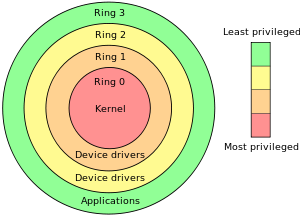
\includegraphics[width=.5\textwidth]{assets/prings.png}
    \caption{Τα διάφορα επίπεδα δικαιωμάτων σε ένα λειτουργικό σύστημα.}
    \label{fig:prings}
\end{figure}


% what each function/macro does

\subsection{Open/Release στον Device Driver}

Η συνάρτηση \src{my\_open} αντιστοιχεί στην αρχικοποίηση της συσκευής.

Αντίστοιχα, στη συνάρτηση \src{release} αποδεσμεύουμε πόρους της συσκευής και τελικά την κλείνουμε.

Ενδεχομένως για μία συσκευή να πρέπει να απαγορεύσουμε ταυτόχρονη χρήση της από πολλές διεργασίες.
Σε αυτή την περίπτωση θα πρέπει η συνάρτηση \src{my\_open} να επιστρέψει τον κωδικό σφάλματος \src{-EBUSY},
ενημερώνοντας έτσι τον χρήστη ο οποίος κάλεσε το system call \src{open} πως δεν μπορεί να χρησιμοποιήσει τη συσκευή.

\begin{file}[open/close device file from userspace (c)]
        \lstinputlisting[language=C]{./assets/open-error.c}
\end{file}

\subsection{Read/Write στον Device Driver}

Όταν μία διεργασία καλέσει τα read/write system calls για το αρχείο το οποίο αντιστοιχεί στη συσκευή μας, το λειτουργικό σύστημα
θα καλέσει αντίστοιχα τις ρουτίνες \src{my\_read}/\src{my\_write}.

Η κλήση τους σε ένα πρόγραμμα C από το user-space θα φαίνεται ως εξής:

\begin{file}[read/write from/to device from userspace (c)]
        \lstinputlisting[language=C]{./assets/rw-user.c}
\end{file}

\begin{itemize}
    

    \item Το read system call μεταφέρει δεδομένα από τη συσκευή σε έναν buffer που βρίσκεται σε user space.
Αυτά μπορεί να είναι δεδομένα όπως το ποιο πλήκτρο πατήθηκε αν μιλάμε για έναν driver πληκτρολογίου.

    \item Το write system call παίρνει δεδομένα τα οποία βρίσκονται σε user-space και τα μεταφέρει στη μνήμη του kernel ώστε να τα χρησιμοποιήσει ο driver της συσκευής.
Αυτά τα δεδομένα μπορεί να είναι κάποιο string που θέλουμε να εμφανιστεί στη κονσόλα.
Η συνάρτηση \src{printf} της βασικής βιβλιοθήκης της C, από μέσα της χρησιμοποιεί το write system call για να εμφανίσει κείμενο στο command line.

\end{itemize}

Και στις δύο περιπτώσεις, εφόσον η συσκευή μας θα έχει επικοινωνία με μία διεργασία χρήστη, πρέπει τα δεδομένα να τα μεταφέρουμε 
και να τα λάβουμε χρησιμοποιώντας τις συναρτήσεις \src{copy\_to\_user} και \src{copy\_from\_user}.

Οι ρουτίνες που θα δημιουργήσουμε στον driver μας (\src{my\_read}, \src{my\_write}) θα επιστρέφουν ένα νούμερο. 

\begin{itemize}
    \item Αν επιστέψουν θετικό αριθμό, θα είναι ο αριθμός των bytes που μεταφέρθηκαν.
    \item Αν επιστρέψουν 0, αυτό σημαίνει πως έχουν μεταφερθεί όλα τα δεδομένα.
    \item Αν επιστρέψουν αρνητικό αριθμό, αυτό σηματοδοτεί κάποιο σφάλμα.
\end{itemize}

Πολλές φορές, η επικοινωνία με μία συσκευή δεν αποτελείται από μία μεγάλη μεταφορά δεδομένων αλλά 
από πολλές μικρές, με την καθεμία να συνεχίζει εκεί που τελείωσε η προηγούμενη.
Για αυτό το λόγο οφείλουμε να λαμβάνουμε υπόψιν το \src{offset} το οποίο δέχεται σαν όρισμα η συνάρτηση \src{my\_read} ή \src{my\_write} του driver μας (παρακάτω φαίνεται το πώς).


\begin{info}[Σημείωση:]
    Τα ορίσματα που περνιούνται στη κάθε συνάρτηση (π.χ. \src{read}) είναι διαφορετικά από το αντίστοιχο system call (\src{ssize\_t \textbf{read(int fd, void *buf, size\_t count)}}).

    Αυτό γίνεται γιατί το λειτουργικό σύστημα μεσολαβεί και κάνει απλούστερη τη διεπαφή.

Για παράδειγμα, στο system call \src{read} ο χρήστης δεν χρειάζεται να περνάει κάποιο συγκεκριμένο offset.
Ωστόσο, όταν πια η κλήση φτάσει στη συσκευή, έχει υπολογιστεί το offset από το οποίο θα συνεχιστεί το διάβασμα των δεδομένων.
Έτσι, ο χρήστης, διαβάζοντας από μια συσκευή, βλέπει μια συνεχή ροή από bytes.
\end{info}

Παραδείγματα υλοποίησης των συναρτήσεων \src{my\_read} και \src{my\_write} όπου γίνεται 
μεταφορά δεδομένα μεταξύ του user-space και ενός buffer που ανήκει στη συσκευή: 

\begin{file}[read/write file operations]
        \lstinputlisting[language=C]{./assets/read-write.c}
\end{file}

\begin{figure}[H]
    \centering
    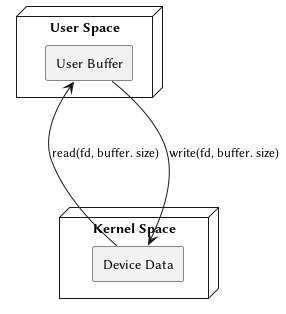
\includegraphics[width=.5\textwidth]{assets/mem-map.png}
    \caption{Η μεταφορά δεδομένων από user-space στη συσκευή μας και το αντίστροφο.}
    \label{fig:drivers}
\end{figure}

\section{Ασκήσεις}

 % Print output of some devices from /dev
 % Register new device    
 % Read from device
 % Write to device (using c program)

% https://github.com/torvalds/linux/blob/master/drivers/input/mousedev.c

\begin{question}
    Βρείτε στον πηγαίο κώδικα του Kernel τους ορισμούς των συμβόλων. Μπορείτε να χρησιμοποιήσετε το εργαλείο αναζήτησης \href{https://elixir.bootlin.com/linux/latest/source}{LXR}.
    \begin{enumerate}
        \item \src{container\_of}
        \item \src{struct file}
        \item \src{struct file\_operations}
    \end{enumerate}
   Εξηγήστε τη σημασία τους. 
\end{question}

\begin{question} % mice
Μία εφαρμογή όπως ο διαχειριστής παραθύρων μας είναι υπεύθυνος για λειτουργίες όπως η εμφάνιση του κέρσορα του ποντικιού.

Όταν εμείς μετακινούμε τη φυσική συσκευή του ποντικιού βλέπουμε τον κέρσορα να μετακινείται.

Ο διαχειριστής παραθύρων δεν γνωρίζει στην πραγματικότητα τίποτα για το ποντίκι μας. 

Κάθε ένα καθορισμένο χρονικό διάστημα η εφαρμογή αυτή ρωτάει το λειτουργικό σύστημα για να δει αν έχει μετακινηθεί το ποντίκι.

Το λειτουργικό σύστημα έχει μεταφράσει την είσοδο από τη συσκευή του ποντικιού σε μία ροή από bytes.
Τα bytes αυτά ακολουθούν ένα συγκεκριμένο \href{https://www.win.tue.nl/~aeb/linux/kbd/scancodes-13.html}{πρωτόκολλο} μέσα από το οποίο περιγράφεται ουσιαστικά η κατεύθυνση στην οποία κινήθηκε το ποντίκι.
Η ροή από bytes φαίνεται στο σύστημά σας ένα απλό αρχείο, το οποίο αν το διαβάσουμε θα δούμε μπορστά μας τη σειρά από bytes που περιγράφουν την κίνηση του ποντικιού μας ανα πάσα στιγμή.

Τελικά, αυτό το αρχείο το διαβάζει ο διαχειριστής παραθύρων και τελικά ζωγραφίζει το ποντίκι στη νέα θέση, όπως θα έπρεπε.

Μπορείτε και τώρα να δείτε αυτό το byte stream χρησιμοποιώντας την παρακάτω εντολή και έπειτα κουνώντας το ποντίκι σας.
(Για πιο όμορφη έξοδο κατεβάστε την εφαρμογή hexdump εκτελώντας \src{sudo apt install hexdump}).

\begin{commandline} 
\begin{verbatim}
$ sudo cat /dev/input/mice
$ sudo cat /dev/input/mice | hexdump # prettier output
\end{verbatim}
\end{commandline}

Τί παρατηρείται;

Έπειτα, εκτελέστε το παρακάτω python script το οποίο ερμηνεύει την έξοδο της συσκευής ποντικιού σαν τριάδες από bytes.

\begin{file}[mouse.py]
        \lstinputlisting[language=C]{../src/device/mouse.py}
\end{file}

Για να εκτελέσετε το script χρησιμοποιήστε την εντολή:

\begin{commandline}
\begin{verbatim}
$ sudo python mouse.py
\end{verbatim}
\end{commandline}


Ποια είναι η έξοδος; Ερμηνεύστε την.

\begin{info}[Σημείωση]
    Μπορείτε να βρείτε την υλοποίηση του driver ποντικιού ο οποίος είναι ενσωματωμένος στο Linux Kernel στο αρχείο
    \src{linux/drivers/input/mouse.c}.
\end{info}


\end{question}


\begin{question}
    Κάντε register ένα character device στο σύστημά σας χρησιμοποιώντας την εντολή \src{mknod}. 
    Δώστε της major αριθμό 42, minor αριθμό 0 και όνομα \src{mydevice}. 

    Προσπαθήστε να γράψετε και να διαβάσετε στη συσκευή. Τί συμβαίνει;

    \begin{info}[Σημείωση]
        Σε αυτή τη συσκευή στη συνέχεια θα αντιστοιχήσουμε τον driver που φτιάχνουμε.
    \end{info}
\end{question}

\begin{question}
   Φτιάξτε ένα kernel module το οποίο θα λειτουργήσει σαν driver της συσκευής που ορίσατε.
   Ο χρήστης θα μπορεί να διαβάσει από και να γράψει στη συσκευή. 
   Συγκεκριμένα, όταν ο χρήστης διαβάζει από τη συσκευή θα παίρνει σαν έξοδο ένα μήνυμα που είναι αποθηκευμένο σε μνήμη που ανήκει στον πυρήνα.
   Όταν γράφει ο χρήστης στη συσκευή θα μπορεί να αλλάξει το μήνυμα το οποίο τυπώνεται.

   Βασιστείτε στον σκελετό που δίνεται στο αρχείο {\bf \src{mychardev.c}}.

    \begin{info}
        Μόλις συμπληρώσετε τον κώδικα. Κάντε τον compile και φορτώστε το module \src{chardev.ko} στον πυρήνα σας.
        Πλέον, θα μπορείτε να αλληλεπιδράσετε με την εικονική συσκευή που φτιάξατε στο προηγούμενο ερώτημα μέσω του driver.
    \end{info}

   Έπειτα, φτιάξτε ένα αρχείο σε όποια γλώσσα προγραμματισμού θέλετε που να επιδεικνύει τη λειτουργία της συσκευής σας.
\end{question}


\section{Πηγές}

\begin{itemize}
    \item \href{https://sysprog21.github.io/lkmpg/}{Linux Kernel Module Programming Guide}
    \item \href{https://lwn.net/Kernel/LDD3/}{Linux Device Drivers}
    \item Operating System Concepts 9th Edition - Silbershatz, Galvin, Gagne (ch. 18)
\end{itemize}

\end{document}
